\section{Recupero password} {
    Nel caso in cui l'utente, al momento del login, avesse dimenticato la propria password per accedere alla piattaforma 
    \platform può recuperarla premendo il link "\textbf{Forgot my password}". 
    \begin{figure}[H]
        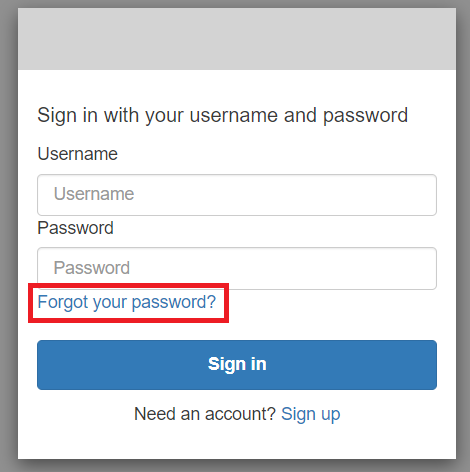
\includegraphics[width=8cm]{sezioni/images/psw-forgot.png}
        \centering
        \caption{Link per recuperare la password durante il login}
    \end{figure}

    Dopo aver cliccato, verrà inviato un codice all'email con cui era avvenuta la registrazione. Sarà neccessario infatti inserire: 
    \begin{itemize}
        \item Code;
        \item New Password;
        \item Enter New Password Again.
    \end{itemize} 
    La nuova password deve rispettare sempre le specifiche generali.
    \begin{figure}[H]
        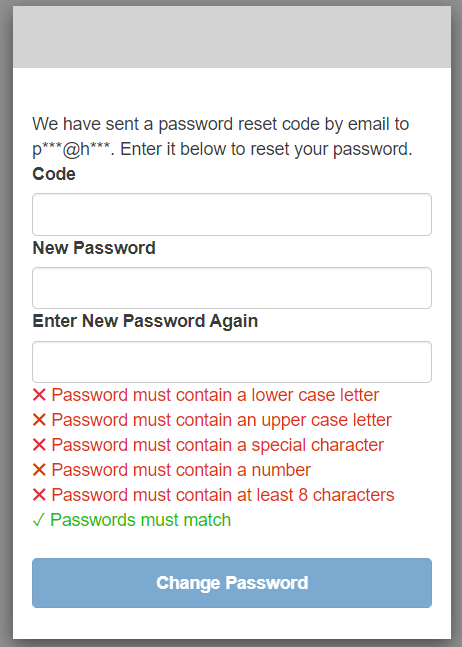
\includegraphics[width=8cm]{sezioni/images/rec-psw.png}
        \centering
        \caption{Campi da inserire durante il recupero password}
    \end{figure}

    \subsection{Credenziale nomeutente errata} {
        Se il campo del nomeutente non viene inserito, il sistema rilverà un errore di questo tipo: infatti non è possibile lasciare 
        tale campo vuoto.

        Se il nomeutente non esiste, verrà rilevato questo tipo di errore: 

        INSERIRE LE FOTO, NON CONOSCO ANCORA BENE LA PROCEDURA
    }
}
